%%
%% Automatically generated file from DocOnce source
%% (https://github.com/hplgit/doconce/)
%%

% #define PREAMBLE

% #ifdef PREAMBLE
%-------------------- begin preamble ----------------------

\documentclass[%
oneside,                 % oneside: electronic viewing, twoside: printing
final,                   % draft: marks overfull hboxes, figures with paths
10pt,french]{article}

\listfiles               %  print all files needed to compile this document

\usepackage{relsize,makeidx,color,setspace,amsmath,amsfonts,amssymb}
\usepackage[table]{xcolor}
\usepackage{bm,ltablex,microtype}

\usepackage[pdftex]{graphicx}

% Packages for typesetting blocks of computer code
\usepackage{fancyvrb,framed,moreverb}

% Define colors
\definecolor{orange}{cmyk}{0,0.4,0.8,0.2}
\definecolor{tucorange}{rgb}{1.0,0.64,0}
\definecolor{darkorange}{rgb}{.71,0.21,0.01}
\definecolor{darkgreen}{rgb}{.12,.54,.11}
\definecolor{myteal}{rgb}{.26, .44, .56}
\definecolor{gray}{gray}{0.45}
\definecolor{mediumgray}{gray}{.8}
\definecolor{lightgray}{gray}{.95}
\definecolor{brown}{rgb}{0.54,0.27,0.07}
\definecolor{purple}{rgb}{0.5,0.0,0.5}
\definecolor{darkgray}{gray}{0.25}
\definecolor{darkblue}{rgb}{0,0.08,0.45}
\definecolor{darkblue2}{rgb}{0,0,0.8}
\definecolor{lightred}{rgb}{1.0,0.39,0.28}
\definecolor{lightgreen}{rgb}{0.48,0.99,0.0}
\definecolor{lightblue}{rgb}{0.53,0.81,0.92}
\definecolor{lightblue2}{rgb}{0.3,0.3,1.0}
\definecolor{lightpurple}{rgb}{0.87,0.63,0.87}
\definecolor{lightcyan}{rgb}{0.5,1.0,0.83}

\colorlet{comment_green}{green!50!black}
\colorlet{string_red}{red!60!black}
\colorlet{keyword_pink}{magenta!70!black}
\colorlet{indendifier_green}{green!70!white}

% Backgrounds for code
\definecolor{cbg_gray}{rgb}{.95, .95, .95}
\definecolor{bar_gray}{rgb}{.92, .92, .92}

\definecolor{cbg_yellowgray}{rgb}{.95, .95, .85}
\definecolor{bar_yellowgray}{rgb}{.95, .95, .65}

\colorlet{cbg_yellow2}{yellow!10}
\colorlet{bar_yellow2}{yellow!20}

\definecolor{cbg_yellow1}{rgb}{.98, .98, 0.8}
\definecolor{bar_yellow1}{rgb}{.98, .98, 0.4}

\definecolor{cbg_red1}{rgb}{1, 0.85, 0.85}
\definecolor{bar_red1}{rgb}{1, 0.75, 0.85}

\definecolor{cbg_blue1}{rgb}{0.87843, 0.95686, 1.0}
\definecolor{bar_blue1}{rgb}{0.7,     0.95686, 1}

%\setlength{\fboxsep}{-1.5mm}  % adjust cod_vpad/pro_vpad background box

%% Background for code blocks (parameter is color name)

%% pro/cod_vpad: gives some vertical padding before and after the text
%% (but has more simplistic code than _cod/pro_tight+cod/pro).
%% pro/cod_vpad can be used to enclose Verbatim or lst begin/end for code.
%% pro/cod calls _pro/cod_tight and has very little vertical padding,
%% used to enclose Verbatim and other begin/end for code.
%% (pro/cod is what the ptex2tex program could produce with the
%% Blue/BlueBar definitions in .ptex2tex.cfg.)

\newenvironment{cod_vpad}[1]{
   \def\FrameCommand{\colorbox{#1}}
   \MakeFramed{\FrameRestore}}
   {\endMakeFramed}

\newenvironment{_cod_tight}[1]{
   \def\FrameCommand{\colorbox{#1}}
   \FrameRule0.6pt\MakeFramed {\FrameRestore}\vskip3mm}
   {\vskip0mm\endMakeFramed}

\newenvironment{cod}[1]{
\bgroup\rmfamily
\fboxsep=0mm\relax
\begin{_cod_tight}{#1}
\list{}{\parsep=-2mm\parskip=0mm\topsep=0pt\leftmargin=2mm
\rightmargin=2\leftmargin\leftmargin=4pt\relax}
\item\relax}
{\endlist\end{_cod_tight}\egroup}

%% Background for complete program blocks (parameter 1 is color name
%% for background, parameter 2 is color for left bar)
\newenvironment{pro_vpad}[2]{
   \def\FrameCommand{\color{#2}\vrule width 1mm\normalcolor\colorbox{#1}}
   \MakeFramed{\FrameRestore}}
   {\endMakeFramed}

\newenvironment{_pro_tight}[2]{
   \def\FrameCommand{\color{#2}\vrule width 1mm\normalcolor\colorbox{#1}}
   \FrameRule0.6pt\MakeFramed {\advance\hsize-2mm\FrameRestore}\vskip3mm}
   {\vskip0mm\endMakeFramed}

\newenvironment{pro}[2]{
\bgroup\rmfamily
\fboxsep=0mm\relax
\begin{_pro_tight}{#1}{#2}
\list{}{\parsep=-2mm\parskip=0mm\topsep=0pt\leftmargin=2mm
\rightmargin=2\leftmargin\leftmargin=4pt\relax}
\item\relax}
{\endlist\end{_pro_tight}\egroup}

\usepackage{minted}
\usemintedstyle{default}

\usepackage[T1]{fontenc}
%\usepackage[latin1]{inputenc}
\usepackage{ucs}
\usepackage[utf8x]{inputenc}

\usepackage{lmodern}         % Latin Modern fonts derived from Computer Modern

% Hyperlinks in PDF:
\definecolor{linkcolor}{rgb}{0,0,0.4}
\usepackage{hyperref}
\hypersetup{
    breaklinks=true,
    colorlinks=true,
    linkcolor=linkcolor,
    urlcolor=linkcolor,
    citecolor=black,
    filecolor=black,
    %filecolor=blue,
    pdfmenubar=true,
    pdftoolbar=true,
    bookmarksdepth=3   % Uncomment (and tweak) for PDF bookmarks with more levels than the TOC
    }
%\hyperbaseurl{}   % hyperlinks are relative to this root

\setcounter{tocdepth}{2}  % levels in table of contents

% Tricks for having figures close to where they are defined:
% 1. define less restrictive rules for where to put figures
\setcounter{topnumber}{2}
\setcounter{bottomnumber}{2}
\setcounter{totalnumber}{4}
\renewcommand{\topfraction}{0.95}
\renewcommand{\bottomfraction}{0.95}
\renewcommand{\textfraction}{0}
\renewcommand{\floatpagefraction}{0.75}
% floatpagefraction must always be less than topfraction!
% 2. ensure all figures are flushed before next section
\usepackage[section]{placeins}
% 3. enable begin{figure}[H] (often leads to ugly pagebreaks)
%\usepackage{float}\restylefloat{figure}

% --- fancyhdr package for fancy headers ---
\usepackage{fancyhdr}
\fancyhf{} % sets both header and footer to nothing
\renewcommand{\headrulewidth}{0pt}
\fancyfoot[LE,RO]{\thepage}
% Ensure copyright on titlepage (article style) and chapter pages (book style)
\fancypagestyle{plain}{
  \fancyhf{}
  \fancyfoot[C]{{\footnotesize \copyright\ 2020, Ahmed Ammar. Released under CC Attribution 4.0 license}}
%  \renewcommand{\footrulewidth}{0mm}
  \renewcommand{\headrulewidth}{0mm}
}
% Ensure copyright on titlepages with \thispagestyle{empty}
\fancypagestyle{empty}{
  \fancyhf{}
  \fancyfoot[C]{{\footnotesize \copyright\ 2020, Ahmed Ammar. Released under CC Attribution 4.0 license}}
  \renewcommand{\footrulewidth}{0mm}
  \renewcommand{\headrulewidth}{0mm}
}

\pagestyle{fancy}


\usepackage{framed,wrapfig}

% --- begin definitions of admonition environments ---

% Admonition style "grayicon" has colored background, no frame, and an icon
% Admon "notice"
\definecolor{grayicon_notice_background}{rgb}{0.91,0.91,0.91}
% \fboxsep sets the space between the text and the box
\newenvironment{noticeshaded}
{\def\FrameCommand{\fboxsep=3mm\colorbox{grayicon_notice_background}}
 \MakeFramed {\advance\hsize-\width \FrameRestore}}{\endMakeFramed}

\newenvironment{notice_grayiconadmon}[1][À noter]{
\begin{noticeshaded}
\noindent
\begin{wrapfigure}{l}{0.07\textwidth}
\vspace{-13pt}

\includegraphics[width=0.07\textwidth]{latex_figs/small_gray_notice}
\end{wrapfigure} \textbf{#1}\par
\nobreak\noindent\ignorespaces
}
{
\end{noticeshaded}
}

% Admonition style "grayicon" has colored background, no frame, and an icon
% Admon "summary"
\definecolor{grayicon_summary_background}{rgb}{0.91,0.91,0.91}
% \fboxsep sets the space between the text and the box
\newenvironment{summaryshaded}
{\def\FrameCommand{\fboxsep=3mm\colorbox{grayicon_summary_background}}
 \MakeFramed {\advance\hsize-\width \FrameRestore}}{\endMakeFramed}

\newenvironment{summary_grayiconadmon}[1][Résumé]{
\begin{summaryshaded}
\noindent
\begin{wrapfigure}{l}{0.07\textwidth}
\vspace{-13pt}
\includegraphics[width=0.07\textwidth]{latex_figs/small_gray_summary}
\end{wrapfigure} \textbf{#1}\par
\nobreak\noindent\ignorespaces
}
{
\end{summaryshaded}
}

% Admonition style "grayicon" has colored background, no frame, and an icon
% Admon "warning"
\definecolor{grayicon_warning_background}{rgb}{0.91,0.91,0.91}
% \fboxsep sets the space between the text and the box
\newenvironment{warningshaded}
{\def\FrameCommand{\fboxsep=3mm\colorbox{grayicon_warning_background}}
 \MakeFramed {\advance\hsize-\width \FrameRestore}}{\endMakeFramed}

\newenvironment{warning_grayiconadmon}[1][Attention]{
\begin{warningshaded}
\noindent
\begin{wrapfigure}{l}{0.07\textwidth}
\vspace{-13pt}

\includegraphics[width=0.07\textwidth]{latex_figs/small_gray_warning}
\end{wrapfigure} \textbf{#1}\par
\nobreak\noindent\ignorespaces
}
{
\end{warningshaded}
}

% Admonition style "grayicon" has colored background, no frame, and an icon
% Admon "question"
\definecolor{grayicon_question_background}{rgb}{0.91,0.91,0.91}
% \fboxsep sets the space between the text and the box
\newenvironment{questionshaded}
{\def\FrameCommand{\fboxsep=3mm\colorbox{grayicon_question_background}}
 \MakeFramed {\advance\hsize-\width \FrameRestore}}{\endMakeFramed}

\newenvironment{question_grayiconadmon}[1][Question]{
\begin{questionshaded}
\noindent
\begin{wrapfigure}{l}{0.07\textwidth}
\vspace{-13pt}
\includegraphics[width=0.07\textwidth]{latex_figs/small_gray_question2}
\end{wrapfigure} \textbf{#1}\par
\nobreak\noindent\ignorespaces
}
{
\end{questionshaded}
}

% Admonition style "grayicon" has colored background, no frame, and an icon
% Admon "block"
\definecolor{grayicon_block_background}{rgb}{0.91,0.91,0.91}
% \fboxsep sets the space between the text and the box
\newenvironment{blockshaded}
{\def\FrameCommand{\fboxsep=3mm\colorbox{grayicon_block_background}}
 \MakeFramed {\advance\hsize-\width \FrameRestore}}{\endMakeFramed}

\newenvironment{block_grayiconadmon}[1][Block]{
\begin{blockshaded}
\noindent
 \textbf{#1}\par
\nobreak\noindent\ignorespaces
}
{
\end{blockshaded}
}

% --- end of definitions of admonition environments ---

% prevent orhpans and widows
\clubpenalty = 10000
\widowpenalty = 10000

\newenvironment{doconceexercise}{}{}
\newcounter{doconceexercisecounter}
% --- begin definition of \listofexercises command ---
\makeatletter
\newcommand\listofexercises{\section*{List of Exercices}
\@starttoc{loe}
}
\newcommand*{\l@doconceexercise}{\@dottedtocline{0}{0pt}{6.5em}}
\makeatother
% --- end definition of \listofexercises command ---



% ------ header in subexercises ------
%\newcommand{\subex}[1]{\paragraph{#1}}
%\newcommand{\subex}[1]{\par\vspace{1.7mm}\noindent{\bf #1}\ \ }
\makeatletter
% 1.5ex is the spacing above the header, 0.5em the spacing after subex title
\newcommand\subex{\@startsection{paragraph}{4}{\z@}%
                  {1.5ex\@plus1ex \@minus.2ex}%
                  {-0.5em}%
                  {\normalfont\normalsize\bfseries}}
\makeatother


% --- end of standard preamble for documents ---


% insert custom LaTeX commands...

\raggedbottom
\makeindex
\usepackage[totoc]{idxlayout}   % for index in the toc
\usepackage[nottoc]{tocbibind}  % for references/bibliography in the toc

%-------------------- end preamble ----------------------

\begin{document}

% matching end for #ifdef PREAMBLE
% #endif

\newcommand{\exercisesection}[1]{\subsection*{#1}}


% ------------------- main content ----------------------



% ----------------- title -------------------------

\thispagestyle{empty}

\begin{center}
{\LARGE\bf
\begin{spacing}{1.25}
TD N°4 : Intégration numérique
\end{spacing}
}
\end{center}

% ----------------- author(s) -------------------------

\begin{center}
{\bf Ahmed Ammar (\texttt{ahmed.ammar@fst.utm.tn})}
\end{center}

    \begin{center}
% List of all institutions:
\centerline{{\small Institut Préparatoire aux Études Scientifiques et Techniques, Université de Carthage.}}
\end{center}
    
% ----------------- end author(s) -------------------------

% --- begin date ---
\begin{center}
Feb 11, 2020
\end{center}
% --- end date ---

\vspace{1cm}


\tableofcontents


\vspace{1cm} % after toc



% !split


% --- begin exercise ---
\begin{doconceexercise}
\refstepcounter{doconceexercisecounter}

\exercisesection{Exercice \thedoconceexercisecounter: Vitesse d'une fusée}


On lance une fusée verticalement du sol et l’on mesure pendant les premières 80 secondes l'accélération $\gamma$:


\begin{quote}
\begin{tabular}{lccccccccc}
\hline
\multicolumn{1}{l}{ t[s] } & \multicolumn{1}{c}{ 0 } & \multicolumn{1}{c}{ 10 } & \multicolumn{1}{c}{ 20 } & \multicolumn{1}{c}{ 30 } & \multicolumn{1}{c}{ 40 } & \multicolumn{1}{c}{ 50 } & \multicolumn{1}{c}{ 60 } & \multicolumn{1}{c}{ 70 } & \multicolumn{1}{c}{ 80 } \\
\hline
$\gamma$ [m $s^{-2}$] & 30 & 31.63 & 33.44 & 35.47 & 37.75 & 40.33 & 43.29 & 46.70 & 50.67 \\
\hline
\end{tabular}
\end{quote}

\noindent
Calculer la vitesse $V$ de la fusée à l’instant $t=80 \ s$, par la méthode des trapèzes.


% --- begin solution of exercise ---
\paragraph{Solution.}
On sait que l’accélération $\gamma$ est la dérivée de la vitesse $V$, donc,
\begin{align*}
V(t) &= \int_0^t \gamma(s) ds \\
I &= V(80) = \int_0^{80} \gamma(s) ds
\end{align*}
Calculons $I$ par la méthode des trapèzes. Ici, d’après le tableau des valeurs, $h = 10$.

\begin{equation*}
I \approx h \left[\frac{1}{2}f(x_0) + \sum_{i=1}^{n-1}f(x_i) + \frac{1}{2}f(x_n) \right]
\end{equation*}
\begin{align*}
I &\approx 10 \left[\frac{1}{2} \times 30 + \frac{1}{2} \times 50.67 + 31.63 + 33.44 + \ldots + 46.70 \right] \\
  &\approx 3089.45 \quad ms^{-1}
\end{align*}
\begin{cod}{cbg_gray}\begin{minted}[fontsize=\fontsize{9pt}{9pt},linenos=false,mathescape,baselinestretch=1.0,fontfamily=tt,xleftmargin=2mm]{python}
h = 10
I = 0.5 * (30 + 50.67) # 1/2 * [f(x0) + f(xn)]
fx = [31.63,33.44,35.47,37.75,40.33,43.29,46.70] # f(x1) ---> f(xn-1)
for i in range(len(fx)):
    I+= fx[i]
I*=h
print(I, "ms^-1")

\end{minted}
\end{cod}
\noindent

% --- end solution of exercise ---

\end{doconceexercise}
% --- end exercise ---


% !split


% --- begin exercise ---
\begin{doconceexercise}
\refstepcounter{doconceexercisecounter}

\exercisesection{Exercice \thedoconceexercisecounter: Valeur approchée de $\pi$}


Étant donnée l'égalité:
\begin{equation}
\pi = 4 \left( \int_0^\infty e^{-x^2} dx \right)^2 = 4 \left( \int_0^{10} e^{-x^2} dx + \epsilon \right)^2
\end{equation}
avec $0 < \epsilon < 10^{−44}$ , utiliser la méthode des trapèzes composite à $10$ intervalles pour estimer la valeur de $\pi$.


% --- begin solution of exercise ---
\paragraph{Solution.}
La méthode des trapèzes composite à $n$ intervalles pour calculer l’intégrale d’une fonction f sur l’intervalle $[a, b]$ s’écrit
\begin{equation*}
\int_a^b f(x)\,dx \approx h \left[\frac{1}{2}f(x_0) + \sum_{i=1}^{n-1}f(x_i) + \frac{1}{2}f(x_n) \right]
\end{equation*}
avec $h = \frac{b-a}{n}$ et $x_i = a + ih,\quad i = 0,1,\ldots,n$

Ici on a $f (x) = e^{-x}$ , $a = 0$, $b = 10$, $n = 10$ d’où $h = 1$ et on obtient
\begin{equation*}
I \approx \frac{1}{2} + \sum_{i=1}^{9} e^{-i} + \frac{1}{2e^{100}} = \frac{1}{2} + \frac{1}{e} + \frac{1}{e^{4}} + \frac{1}{e^{9}} + \frac{1}{e^{16}} + \frac{1}{e^{25}} + \frac{1}{e^{36}} + \frac{1}{e^{49}} + \frac{1}{e^{64}} + \frac{1}{e^{81}} + \frac{1}{2e^{100}}
\end{equation*}
ainsi en utilisant la fonction \texttt{trapeze(f,a,b,n)} du module \Verb!trapeze_integral.py! décrite dans le cours comme suit
\begin{cod}{cbg_gray}\begin{minted}[fontsize=\fontsize{9pt}{9pt},linenos=false,mathescape,baselinestretch=1.0,fontfamily=tt,xleftmargin=2mm]{python}
from trapeze_integral import trapeze
from math import exp
f = lambda x: exp(-x**2)
I = trapeze(f, 0, 10, 10)
print(4*I**2)
\end{minted}
\end{cod}
\noindent
on obtient $\pi \approx 4I^2 = 3.14224265994$.

% --- end solution of exercise ---

\end{doconceexercise}
% --- end exercise ---


% !split


% --- begin exercise ---
\begin{doconceexercise}
\refstepcounter{doconceexercisecounter}

\exercisesection{Exercice \thedoconceexercisecounter: Intégration adaptative}

\label{ex:adaptatif}

Supposons que nous voulons utiliser la méthode des trapèzes ou du point milieu pour calculer une intégrale $\int_a^b f(x)dx$ avec une erreur inférieure à une tolérance prescrite $\epsilon$. Quelle est la taille appropriée de $n$?

Pour répondre à cette question, nous pouvons entrer une procédure itérative où nous comparons les résultats produits par $n$ et $2n$ intervalles, et si la différence est inférieure à $\epsilon$, la valeur correspondant à $2n$ est retournée. Sinon, nous avons $n$ et répétons la procédure.

% --- begin hint in exercise ---

\paragraph{Indication.}
Il peut être une bonne idée d'organiser votre code afin que la fonction \Verb!integration_adaptive! peut être utilisé facilement dans les programmes futurs que vous écrivez.

% --- end hint in exercise ---


\subex{a)}
Écrire une fonction \Verb!integration_adaptive(f, a, b, eps, method="midpoint")! qui implémente l'idée ci-dessus (\texttt{eps} correspond à la tolérance $\epsilon$, et la méthode peut être \texttt{midpoint} ou \texttt{trapeze}).


% --- begin solution of exercise ---
\paragraph{Solution.}
En facilitant les réponses à l'ensemble de cet exercice, ainsi qu'en préparant l'utilisation facile de l'intégration adaptative dans les futurs programmes, nous organisons le codage des tâches a, b et c en un seul fichier, ce qui en fait un module. Le code se lit alors:

\begin{pro}{cbg_gray}{bar_gray}\begin{minted}[fontsize=\fontsize{9pt}{9pt},linenos=false,mathescape,baselinestretch=1.0,fontfamily=tt,xleftmargin=2mm]{python}
## NOM DU PROGRAMME: integration_adaptive.py
#% IMPORTATION
from numpy import linspace, zeros, sqrt
from trapeze_integral import trapeze
from midpoint_integral import midpoint

def integration_adaptative(f, a, b, eps, method='midpoint'):
    '''
    Question a)
    '''
    n_limit = 1000000  # Juste un choix (utilisé pour éviter la boucle inf)
    n = 2
    if method == 'trapeze':
        integral_n  = trapeze(f, a, b, n)
        integral_2n = trapeze(f, a, b, 2*n)
        diff = abs(integral_2n - integral_n)
        while (diff > eps) and (n < n_limit):
            integral_n  = trapeze(f, a, b, n)
            integral_2n = trapeze(f, a, b, 2*n)
            diff = abs(integral_2n - integral_n)
            n *= 2
    elif method == 'midpoint':
        integral_n  = midpoint(f, a, b, n)
        integral_2n = midpoint(f, a, b, 2*n)
        diff = abs(integral_2n - integral_n)
        while (diff > eps) and (n < n_limit):
            integral_n  = midpoint(f, a, b, n)
            integral_2n = midpoint(f, a, b, 2*n)
            diff = abs(integral_2n - integral_n)
            n *= 2
    else:
        print('Erreur - intégration adaptative appelée avec un paramètre inconnu')
    # Maintenant, nous vérifions si un n acceptable a été trouvé ou non
    if diff <= eps:   # Succès
        print("L'intégrale calcule: ", integral_2n)
        return n
    else:
        return -n   # Renvoie n négatif pour dire "non trouvé"

def application():
    """Questions b) and c)"""

    g = lambda x: sqrt(x)

#    eps = 1E-1 # Il suffit de basculer entre ces deux valeurs eps
    eps = 1E-10
    a = 0.0 + 0.01  # Si nous ajustons a, sqrt (x) est géré facilement
    b = 2.0
    n = integration_adaptative(g, a, b, eps, 'midpoint')
    if n > 0:
        print('n suffisant est: %d'%(n))
    else:
        print("Aucun n n'a été trouvé dans %d iterations" % (n_limit))
   
    # c) faire un tracé pour le point milieu et les trapèzes
    eps = linspace(1E-1,10E-10,10)
    n_m = zeros(len(eps))
    n_t = zeros(len(eps))
    for i in range(len(n_m)):
        n_m[i] = integration_adaptative(g, a, b, eps[i], 'midpoint')
        n_t[i] = integration_adaptative(g, a, b, eps[i], 'trapeze')

    import matplotlib.pyplot as plt
    plt.figure(figsize=(7,5))
    plt.plot(eps,n_m,'b-', label = "méthode du point milieu")
    plt.plot(eps,n_t,'r-',  label = "méthode des trapèzes")
    plt.xlabel(r'$\epsilon$')
    plt.ylabel('n')
    plt.xscale("log")
    plt.legend()
    plt.show()

if __name__ == '__main__':
    application()
\end{minted}
\end{pro}
\noindent

% --- end solution of exercise ---

\subex{b)}
Testez la méthode sur $g(x) = \int_0^2\sqrt{x}dx$ pour $\epsilon = 10^{−1},10^{−10}$ et notez l'erreur exacte.


% --- begin solution of exercise ---
\paragraph{Solution.}
Voir le code ci-dessus. Notez que, dans notre code suggéré, il est prévu que le programmeur bascule entre les deux valeurs epsilon en utilisant des commentaires, c'est-à-dire en ajoutant/supprimant \Verb!#!. Cela peut bien sûr être évité, si cela est souhaitable, en demandant à l'utilisateur d'entrer un valeur d'epsilon.

% --- end solution of exercise ---

\subex{c)}
Faites un tracé de $n$ en fonction de $\epsilon \in [10^{-1}, 10^{-10}]$ pour $\int_0^2\sqrt{x}dx$. Utilisez l'échelle logarithmique pour $\epsilon$.


\begin{figure}[!ht]  % fig:eps
  \centerline{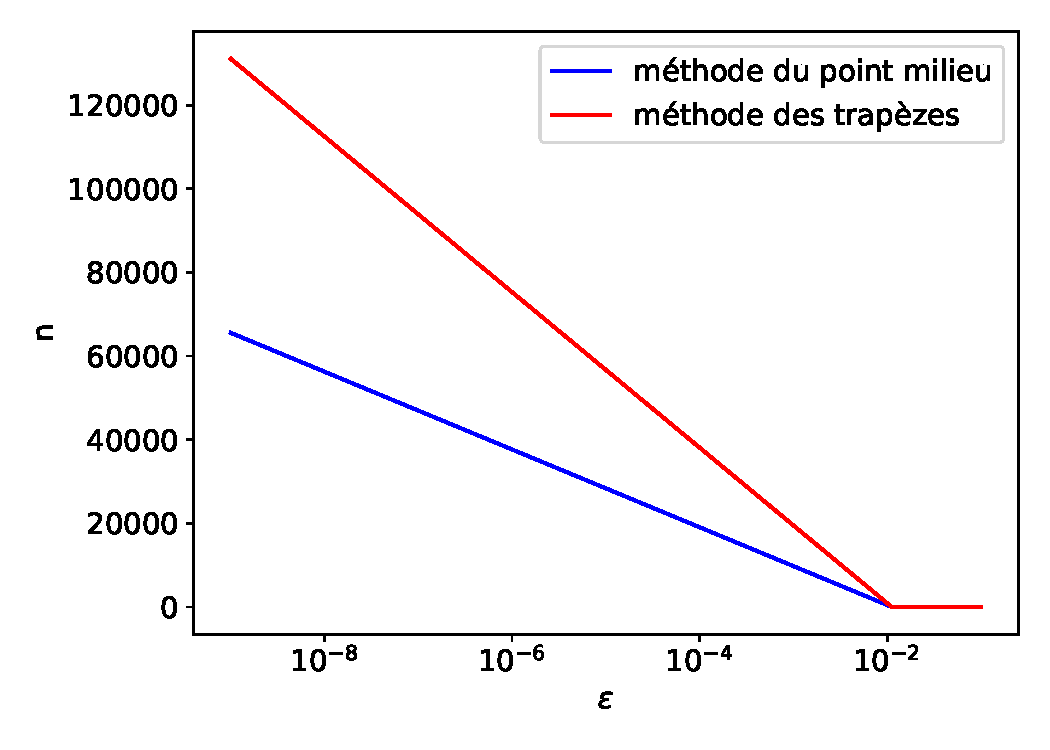
\includegraphics[width=0.7\linewidth]{imgs/eps.pdf}}
  \caption{
  Affichage de n en fonction de $\epsilon$ lorsque $\int_0^2\sqrt{x}dx$ est calculé par la méthode du point milieu (bleu) et la méthode des trapèzes (rouge). \label{fig:eps}
  }
\end{figure}
%\clearpage % flush figures fig:eps



% --- begin solution of exercise ---
\paragraph{Solution.}
La figure~\ref{fig:eps} montre que plus la valeur d'epsilon est stricte, plus la différence entre les méthodes du point milieu et des trapèzes est grande. Pour une valeur donnée pour epsilon, la méthode du point milieu se situe dans la tolérance avec moins d'intervalles (valeur inférieure de $n$) que la méthode des trapèzes. Il faut s'y attendre, car la méthode du point milieu est un peu plus précise que la méthode des trapèzes.

Une façon de produire ce tracé est d'utiliser les lignes de code incluses à la fin de \Verb!integration_adaptive.py! (voir ci-dessus).

% --- end solution of exercise ---


% Closing remarks for this Exercice

\paragraph{Remarques.}
Le type de méthode exploré dans cet exercice est appelé \emph{adaptatif}, car il essaie d'adapter la valeur de n pour répondre à un critère d'erreur donné. La vraie erreur peut très rarement être calculée (car nous ne connaissons pas la réponse exacte au problème de calcul), il faut donc trouver d'autres indicateurs de l'erreur, comme celui ici où les changements de la valeur intégrale, comme le nombre d'intervalles est doublé, est pris pour refléter l'erreur.


\end{doconceexercise}
% --- end exercise ---


% !split


% --- begin exercise ---
\begin{doconceexercise}
\refstepcounter{doconceexercisecounter}

\exercisesection{Exercice \thedoconceexercisecounter: Intégration de x élevé à x}


Considérons l'intégrale
\begin{equation*}
I = \int_0^2 x^x\,dx\thinspace .
\end{equation*}
L'intégrande $x^x$ n'a pas de primitive qui peut être exprimé en termes de fonctions standard (visitez \href{{http://wolframalpha.com}}{\nolinkurl{http://wolframalpha.com}} et tapez \Verb!integral x^x dx from 0 to 2! pour vous convaincre que notre affirmation est juste. Notez que Wolfram alpha vous donne une réponse, mais cette réponse est une approximation, elle n'est pas \emph{exacte}. C'est parce que Wolfram alpha utilise également des méthodes numériques pour arriver à la réponse, comme vous le ferez dans cet exercice). Par conséquent, nous sommes obligés de calculer l'intégrale par des méthodes numériques. Calculez un résultat composé de quatre chiffres.

% --- begin hint in exercise ---

\paragraph{Indication.}
Utilisez des idées de l'exercice~\ref{ex:adaptatif}.

% --- end hint in exercise ---


% --- begin solution of exercise ---
\paragraph{Solution.}
Lorsque la fonction \Verb!integration_adaptive! est disponible, le code peut s'écrire:

\begin{pro}{cbg_gray}{bar_gray}\begin{minted}[fontsize=\fontsize{9pt}{9pt},linenos=false,mathescape,baselinestretch=1.0,fontfamily=tt,xleftmargin=2mm]{python}
## NOM DU PROGRAMME: xtox.py
#% IMPORTATION
from integration_adaptive import integration_adaptative

def f(x):
    return x**x

eps = 1E-4
a = 0.0;  b = 2.0

# Choisir la méthode milieu
n = integration_adaptative(f, a, b, eps, 'midpoint')
if n > 0:
    print('n suffisant est: %d'%(n))
else:
    # Le n négatif est renvoyé pour signaler que la limite supérieure de n 
    # a été dépassée
    print("Aucun n n'a été trouvé dans %d iterations"  % (abs(n)))
\end{minted}
\end{pro}
\noindent

N'oubliez pas que \Verb!integration_adaptive! affiche l'intégrale calculée, donc aucun effort à cet égard n'est requis ici.

L'exécution du programme donne une impression à l'écran montrant comment la différence devient de plus en plus petite à chaque fois. Les deux lignes de l'impression se lisent comme suit:
\begin{cod}{cbg_gray}\begin{minted}[fontsize=\fontsize{9pt}{9pt},linenos=false,mathescape,baselinestretch=1.0,fontfamily=tt,xleftmargin=2mm]{text}
L'intégrale calcule:  2.8338439595776044
n suffisant est: 256
\end{minted}
\end{cod}
\noindent
La valeur calculée peut être comparée à ce que donne Wolfram alpha. N'oubliez pas qu'étant donné que nous n'avons pas calculé l'erreur exacte, nous ne pouvons garantir que le "résultat est correct à quatre chiffres". Cependant, nous avons des raisons de croire que nous "sommes proches". Typiquement, lorsque l'on sait que la mesure d'erreur utilisée n'est pas précise, la tolérance est rendue plus stricte.

% --- end solution of exercise ---

\end{doconceexercise}
% --- end exercise ---


% !split


% --- begin exercise ---
\begin{doconceexercise}
\refstepcounter{doconceexercisecounter}

\exercisesection{Exercice \thedoconceexercisecounter: Orbitales atomiques}


Pour décrire la trajectoire d'un électron autour d'un noyau, une description probabiliste est adoptée : l'électron n'est plus caractérisé par ses coordonnées spatiales mais par sa \emph{probabilité de présence} en un point de l'espace.

Pour simplifier le problème, on considérera que cette probabilité de présence ne dépend que de la variable $r$, distance entre l'électron et le centre du noyau. Pour une orbitale $1s$, la probabilité de trouver l'électron entre les rayons $r_1$ et $r_2$ s'écrit :
\begin{align*}
P_{s1} = \int_{r_1}^{r_2} \underbrace{4 \times \frac{r^2}{a_0^3} \times e^{-2 \times \frac{r}{a_0}}}_\text{densité radiale} dr
\end{align*}
avec $a_0 = 0.529$ $\AA$, appelé le rayon de Bohr.

La densité radiale, représentée dans la figure~\ref{fig:D_rad}, est maximale pour $r = a_0$. Ce rayon qui maximise la densité radiale est appelé le \emph{rayon orbitalaire}.

\begin{notice_grayiconadmon}[À noter]
Dans ce problème, les distances seront conservées en Angström.
\end{notice_grayiconadmon} % title: À noter




\begin{figure}[!ht]  % fig:D_rad
  \centerline{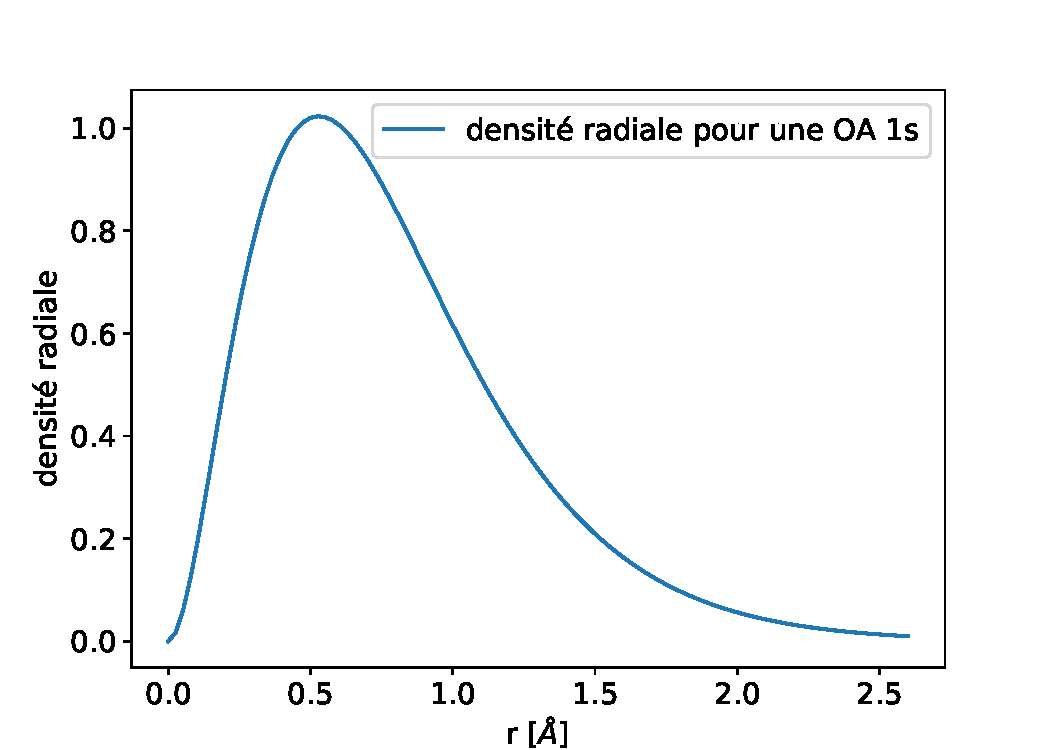
\includegraphics[width=0.7\linewidth]{imgs/densite_radiale.pdf}}
  \caption{
  Densité radiale pour une orbitale atomique 1s. \label{fig:D_rad}
  }
\end{figure}
%\clearpage % flush figures fig:D_rad



\subex{a)}
Définir une fonction \Verb!densite_radiale()!, définie entre $0$ et $\infty$ qui prend comme paramètre variable un rayon $r$ et comme paramètre par défaut $a_0 = 0.529$ $\AA$ et renvoie la valeur $4 \times \frac{r^2}{a_0^3} \times e^{-2 \times \frac{r}{a_0}}$.

\subex{b)}
Tracer la densité radiale pour $r \in [0, 2.6] \quad \AA$, afin d'obtenir le même graphique sur la figure~\ref{fig:D_rad}.

\subex{c)}
On souhaite déterminer la probabilité de présence de l'électron entre $0$ et $a_0$. Évaluer cette probabilité à l'aide de $100$ rectangles. On pourra vérifier que la réponse obtenue est proche de $0.32$.

\subex{d)}
Déterminer le nombre entier $n$, tel que l'électron ait une probabilité supérieure ou égale à $90 \%$ de se trouver entre $0$ et $n*a_0$.

\subex{e)}
On souhaite désormais évaluer la probabilité de trouver l'électron proche du rayon de Bohr, c'est-à-dire entre $0.9*a_0$ et $1.1*a_0$. Évaluer cette probabilité à l'aide de 100 rectangles.

\subex{f)}
D'après la valeur obtenue à la question précédente, que penser de la description des trajectoires des électrons par orbite autour du noyau ?

\begin{notice_grayiconadmon}[À noter]
On répondra en commentaire dans le programme.
\end{notice_grayiconadmon} % title: À noter




% --- begin solution of exercise ---
\paragraph{Solution.}
La solution de l'exercice est dans le programme python suivant:
\begin{pro}{cbg_gray}{bar_gray}\begin{minted}[fontsize=\fontsize{9pt}{9pt},linenos=false,mathescape,baselinestretch=1.0,fontfamily=tt,xleftmargin=2mm]{python}
## NOM DU PROGRAMME: OrbitalesAtomiques.py
#% IMPORTATION
import numpy as np
import matplotlib.pyplot as plt
from midpoint_integral import midpoint
# a) 
def densite_radiale(r, a0 = 0.529):
    return 4 * (r**2/a0**3) * np.exp(-2*(r/a0))
# b)
r = np.linspace(0,2.6, 100)

plt.figure(figsize=(7,5))
plt.plot(r, densite_radiale(r), label = "densité radiale pour une OA 1s")
plt.xlabel("r "+r"$[\AA]$")
plt.ylabel("densité radiale")
plt.legend()
plt.show()

# c) probabilité de présence de l’électron entre 0 et a0
a0 = 0.529
Pa0 = midpoint(densite_radiale, 0, a0, 100)
print("La probabilité de présence de l’électron entre 0 et a0 est: ", Pa0)

# d) rayon moyen de l'OA 1s

for n in range(21):
    Prn = midpoint(densite_radiale, 0, n*a0, 100)
    if Prn >= 0.90:
        print("n = %d, Pr%d = %.4f"%(n,n,Prn))
    
'''
r90 = 3*a0. On dit donc que la rayon moyen de l'OA 1s de l'atome d'hydrogène 
est une sphère de rayon 3*a0, soit à peu près 1.6 Å.
'''

# e)
Pr = midpoint(densite_radiale, 0.9*a0, 1.1*a0, 100)
print("La probabilité de présence de l’électron entre 0.9*a0 et 1.1*a0 est: ", Pr)

# La probabilité de présence de l’électron entre 0.9*a0 et 1.1*a0 est:  0.10790737203009312

# f) Conclusion

'''
* La densité radiale de probabilité de présence est maximale 
pour r = a0 (rayon de Bohr) On dit que c'est le rayon le plus probable.

* Ce résultat est trompeur, car entre 0.9*a0  et 1.1*a0, la probabilité de présence
de l'électron n'est que de 11%.

* l'atome d'hydrogène est une sphère de rayon 3*a0, soit à peu près 1.6 Å.

* La probabilité de présence de l’électron 1s est plus élevée à l’extérieur 
de l’orbite de Bohr. 
'''
\end{minted}
\end{pro}
\noindent

% --- end solution of exercise ---

\end{doconceexercise}
% --- end exercise ---


% ------------------- end of main content ---------------

% #ifdef PREAMBLE
\end{document}
% #endif

